Real-world planning applications frequently involve continuous resources (e.g. fuel, energy and money) and can be modelled as Hybrid Markov Decision Processes (HMDPs). 
%Most existing exact solutions for HMDPs make restrictive assumptions of hyper-rectangular partitions~(\cite{feng04,li05}) or use approximate projections on continuous base functions~(\cite{li05,kveton06HALP}).
Symbolic dynamic programming (SDP)~(\cite{sanner11,zamani12}) provides an exact solution for HMDPs with discrete noise, using the eXtended Algebraic Decision Diagram (XADD) representation.
The XADD structure is a generalisation of the algebraic decision diagram (ADD)~\cite{bahar93add} to represent functions of both discrete and continuous variables.
Decision nodes may contain boolean variables or inequalities between expressions containing continuous variables.
Terminal nodes contain an expression on the continuous variables which could be evaluated to a real number. An example of XADD is shown in Figure \ref{fig:exampleDD}.

%%%%%%%%%%%%%%%%%%%%%%%%%%%%%%%%%%%%%%%%%%%%%%%%
\begin{figure}[t!]
\hspace{-5mm}
\begin{minipage}{0.25\textwidth}
\center
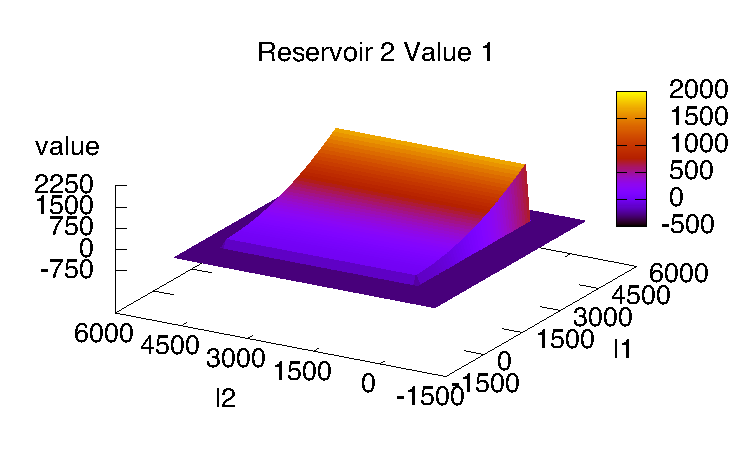
\includegraphics[width=\textwidth, height=0.75\textwidth]{figures/reservoir2Value1/reservoir2Value1.pdf} 
\end{minipage}
\hspace{-2mm}
\begin{minipage}{0.25\textwidth}
\center
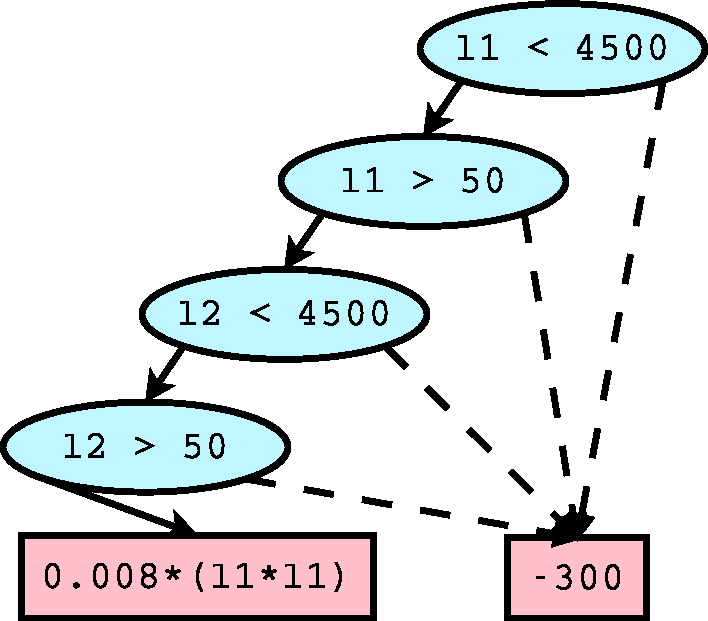
\includegraphics[width=\textwidth, height=0.65\textwidth]{figures/reservoir2Value1/reservoir2Value1DD.pdf}
\end{minipage}\vspace{-3mm}\\
\caption{\footnotesize Ilustration of a local reward function from the \Invent domain: \emph{(left)} graphical plot; \emph{(right)} XADD representation. Blue ovals represent internal nodes, pink rectangles represent terminal nodes. The $true$ branches are solid lines, $false$ are dashed.}
\label{fig:exampleDD}
\vspace{-6mm}
\end{figure}
%%%%%%%%%%%%%%%%%%%%%%%%%%%%%%%%%%%%%%%%%%%%%%%%
\vspace{1mm}
\paragraph{\bf Example 1 - \Invent ~\cite{scarf2002} \label{ex1}}
\textit{An inventory control problem, consists of determining what itens from the inventory should be ordered and how much to order of each. There is a continuous variables $x_i$ for each item $i$ and a single action $order$ with continuous parameters $dx_i$ for each item. There is a fixed limit $L$ for the maximum number of items in the warehouse and a limit $l_i$ for how much of an item can be ordered in a single action. The items are sold according to a stochastic demand, modelled by boolean variables $d_i$ that represent whether demand is high ($Q$ units) or low ($q$ units) for item $i$. A reward is given for each sold item, but there are linear costs for items ordered and held in the warehouse. For item $i$, the reward is as follows:
\begin{align*}
\small
R_{i} (x_i, d_i, dx_i)=
\begin{cases}
  \text{if }  d_i \wedge x_i + dx_i > Q &\hspace{-2mm} : Q - 0.1x_i - 0.3dx_i\\ 
  \text{if }  d_i \wedge x_i + dx_i < Q &\hspace{-2mm} : 0.7x_i - 0.3dx_i\\ 
  \text{if }  \neg d_i \wedge x_i + dx_i > q &\hspace{-2mm} : q - 0.1x_i - 0.3dx_i\\ 
  \text{if }  \neg d_i \wedge x_i+dx_i < q &\hspace{-2mm} : 0.7x_i - 0.3dx_i\\ 
\end{cases}
\end{align*}
}

A drawback of the SDP solution for HMDPs is the overhead of computing a complete optimal policy even for problems where the initial state is known and a partial solution would be sufficient. Though there exist previous solutions to HMDPs that use initial state information, they require monotonic resource consumption and aren't as general as SDP~\cite{meuleau09HAO}.

The Real Time Dynamic Programming (RTDP) algorithm is considered a state-of-the-art solver for MDPs~(\cite{Barto95RTDP,kolobov12GOURMAND}). It combines initial state information and a value function heuristic with asynchronous state value updates to generate an optimal partial policy closed for the relevant states, i.e., states reachable from the initial state following the optimal policy.

In this work, we propose a new HMDP solver, named Real Time Symbolic Dynamic Programming (RTSDP), which uses the symbolic representation of XADDs combined with RTDP to perform a heuristic search with asynchronous SDP, i.e. dynamic programming updating only some parts of the state space.
As the XADD representation naturally factors the state-space into regions with the same continuous expressions, we perform \emph{region based updates} that improve the value function not only for the current state, but \emph{generalize this update to all states in the same region}. We claim that region updates promote better reusability of previous updates, improving the search efficiency. 

Our algorithm is empirically tested on two challenging types of domains: nonlinear domains in which the action set is finite but the transition dynamic is nonlinear on state variables; and continuous actions domains in which actions have continuous parameters and the dynamics are linear on both state and parameter variables.
We empirically show that, given an initial state, RTSDP can solve these HMDP problems faster and using less memory than SDP.
